\documentclass{article}
\usepackage[utf8]{inputenc}
\usepackage[T1]{fontenc}
\usepackage[english,brazil]{babel}
\usepackage{graphicx}
\usepackage{lmodern}
\usepackage{amsmath}
\usepackage[top=3cm,left=3cm,bottom=2cm,right=2cm]{geometry}
\usepackage{hyperref}
\usepackage{icomma}
\usepackage{gensymb}

\hypersetup{
	unicode=true,
	colorlinks=true,
	linkcolor=black,
	citecolor=black,
}

\title{Memorial de cálculo - Bancada de ensino de Aerogeradores}
\author{Henrique Baron}
\bibliographystyle{acm}
\graphicspath{{./imagens/}}

\let\oldforeignlanguage\foreignlanguage
\renewcommand\foreignlanguage[2]{\oldforeignlanguage{#1}{\emph{#2}}}

\begin{document}
	\maketitle
	
	\section{Equações gerais}
	Esta seção descreve as equações que são utilizadas de modo geral como base para os cálculos e modelos posteriores.
	
	\paragraph{Potência do vento}
	A potência do vento é dada por
	\begin{equation} \label{eqn:pot-vento}
		P = \frac{1}{2}\,\rho\,A\,v^3 \text{.}
	\end{equation}
	\begin{description}
		\item[$ P $] Potência do vento, em watts;
		\item[$ \rho $] Densidade do ar, em quilogramas por metro cúbico;
		\item[$ A $] Área avaliada (que corresponde à área de varredura das pás do aerogerador), em metros quadrados;
		\item[$ v $] Velocidade do vento, em metros por segundo.
	\end{description}

	\paragraph{Densidade do ar}
	A densidade do ar, que é utilizada no cálculo da potência, é dada por
	\begin{equation}
		\rho = \frac{P_a}{R\,T}
	\end{equation}
	de modo que $ P_a $ corresponde à pressão atmosférica no local, $ R $ é a constante universal dos gases, e $T$ é a temperatura do ar.
	No trabalho desenvolvido, a densidade do ar foi adotada como constante, com o valor de $ 1,225 $ kg/m\textsuperscript{3}.
	
	\paragraph{Razão de velocidade de ponta}
	Chamada em inglês de \emph{\foreignlanguage{english}{tip speed ratio}}, é a razão entre a velocidade tangencial na ponta da pá, $v_{tt}$, e a velocidade do vento $v$, portanto
	\begin{equation} \label{eqn:tsr-definicao}
		\lambda = \frac{v_{tt}}{v} = \frac{\omega_t\,D}{2\,v} \text{.}
	\end{equation}
	\begin{description}
		\item[$\omega_t$] Velocidade angular do rotor, em radianos por segundo;
		\item[$D$] Diâmetro do rotor, em metros.
	\end{description}

	\paragraph{Coeficientes de torque e potência}
	Os coeficientes de torque e potência do aerogerador, adimensionais, são relacionados com a razão de velocidade de ponta pela fórmula
	\begin{equation} \label{eqn:tsr-coeficientes}
		\lambda = \frac{C_p}{C_t} \text{.}
	\end{equation}
	É importante ressaltar que o coeficiente de potência $C_p$ não pode ser maior que $0,59$, obedecendo o \emph{limite de Betz}.

	\paragraph{Potência extraída pelo aerogerador}
	Conforme a definição do \emph{limite de Betz}, o aerogerador não pode extrair toda a potência disponível no vento.
	A quantidade que é extraída pelo aerogerador de fato, definida como $P_t$, é obtida multiplicando-se equação \ref{eqn:pot-vento} pelo coeficiente de potência $C_p$:
	\begin{equation} \label{eqn:pot-extraida-turbina}
		P_t = \frac{1}{2}\rho\,A\,C_p\,v^3 \text{.}
	\end{equation}
	
	\paragraph{Torque na turbina}
	A definição de potência em um eixo $P = T\omega$ pode ser rearranjada para definir o torque no rotor do aerogerador.
	Substituindo nessa definição as equações \ref{eqn:pot-vento} e \ref{eqn:tsr-definicao}, chega-se a
	\begin{equation} \label{eqn:torque-cp}
		T = \frac{\rho\,A\,C_p v^2 D}{4\lambda} \text{,}
	\end{equation}
	e da mesma forma a equação \ref{eqn:tsr-coeficientes} pode ser utilizada para representar o torque em termos do seu coeficiente, $C_t$;
	\begin{equation} \label{eqn:torque-ct}
		T = \frac{\rho\,A\,C_t v^2 D}{4} \text{.}
	\end{equation}
	
	\section{Determinação do coeficiente de potência}
	O coeficiente de potência $C_p$ pode ser aproximado em termos da relação de velocidade de ponta da pá $\lambda$ e do ângulo de passo $\theta$ (em radianos) como \cite{pinto:2014}
	\begin{equation} \label{eqn:aprox-cp}
		C_p \approx 0,22
		\left( \frac{116}{\lambda} - 0,4\theta - 5 \right)
		e^{-12,5/\lambda}
	\end{equation}
	
	Uma representação dessa função para um ângulo $\theta$ igual a zero -- indicando o máximo aproveitamento da pá -- é exibido na Figura \ref{fig:curva-cp-lambda}.
	\begin{figure}[ht]
		\centering
		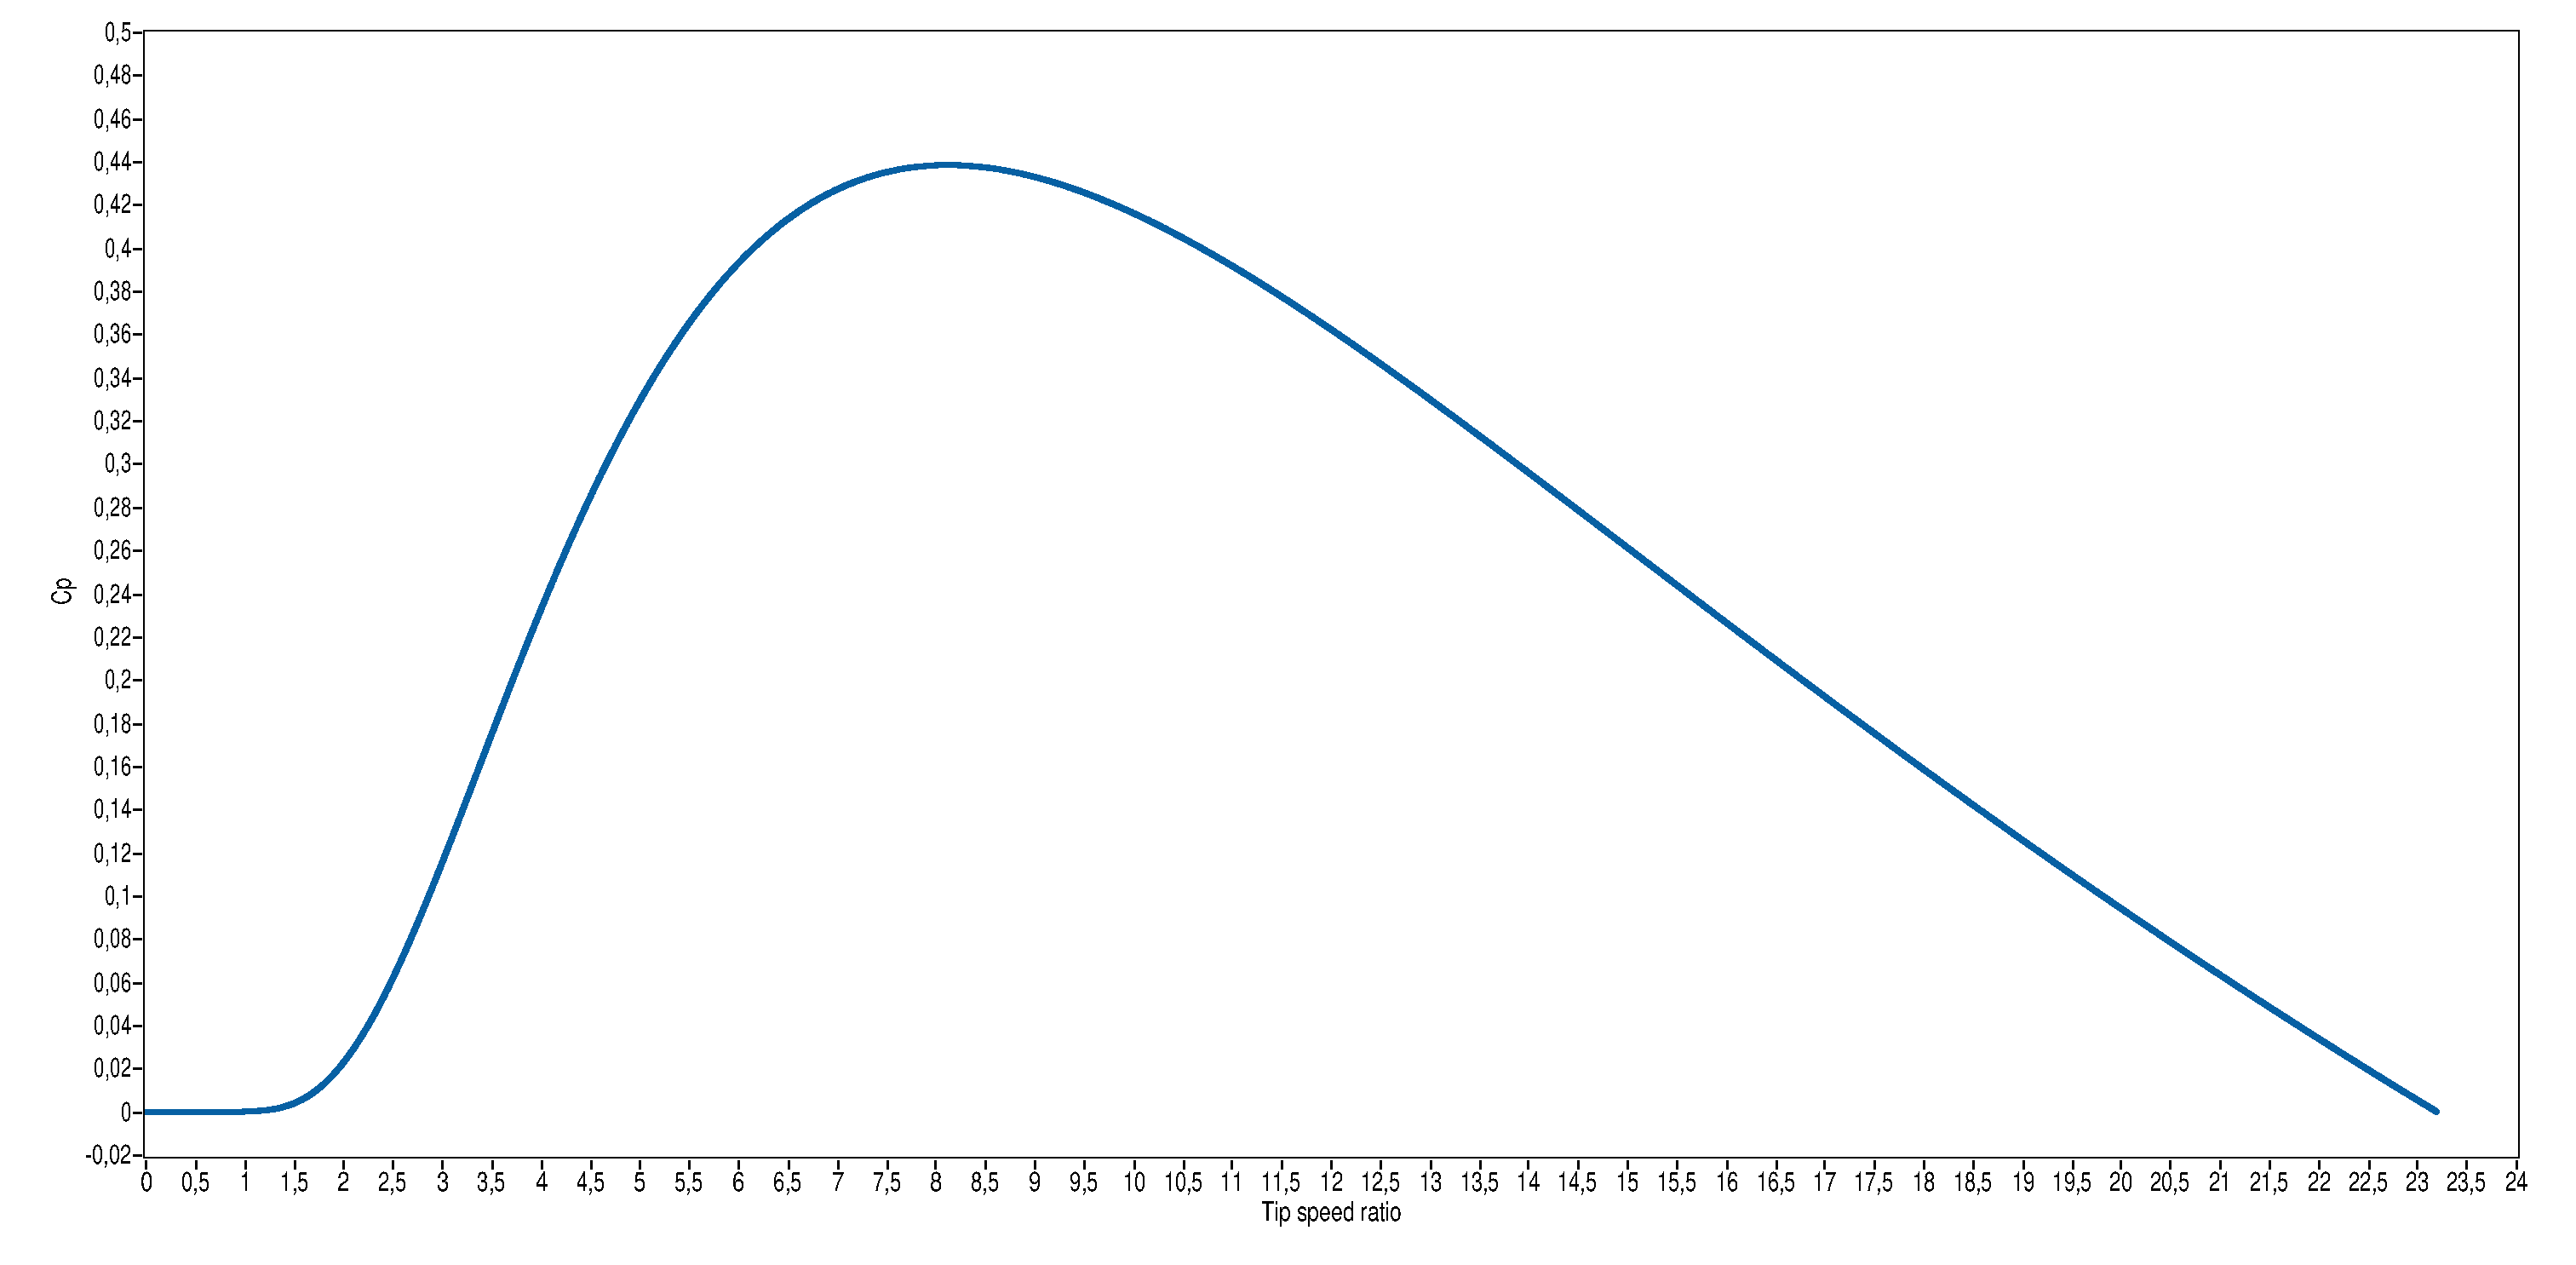
\includegraphics[scale=0.28]{curva-cp-lambda}
		\caption{Coeficiente de potência em relação à razão de velocidade de ponta da pá}
		\label{fig:curva-cp-lambda}
	\end{figure}

	Pela equação, fica visível que um aumento no ângulo de passo $\theta$ provocará uma redução linear no valor de $C_p$, fazendo com que o coeficiente de potência máximo reduza e ocorra em valores menores da relação de velocidade de ponta $\lambda$.
	A resolução desta equação permite também determinar o coeficiente de torque $C_t$, substituindo a equação \ref{eqn:aprox-cp} na equação \ref{eqn:tsr-coeficientes}.
	
	\section{Curva de potência do aerogerador}
	A curva de potência do aerogerador é dividida em quatro zonas \cite{pinto:2014}, como mostra a Figura \ref{fig:zonas-curva-potencia}.
	Pelas zonas pode-se perceber o ponto onde o aerogerador passa a atuar o controle de passo para limitar a potência para que não passe do valor nominal da turbina.
	\begin{figure}[ht]
		\centering
		\includegraphics[scale=0.15]{zonas-curva-potencia.png}
		\caption{Zonas da curva de potência de uma turbina eólica}
		\label{fig:zonas-curva-potencia}
	\end{figure}

	\section{Fundamentos de aerodinâmica}
	Esta seção demonstra os conceitos básicos de aerodinâmica que são utilizados na concepção da turbina do aerogerador.

	\subsection{Dimensões e parâmetros}
	A \figurename\ \ref{fig:diagrama-asa} mostra as dimensões principais de um aerofólio qualquer. 
	Das medidas identificadas, a mais importante a ser observada é a \emph{linha de corda}, identificada na imagem como \foreignlanguage{english}{chord line}.

	\begin{figure}[ht]
		\centering
		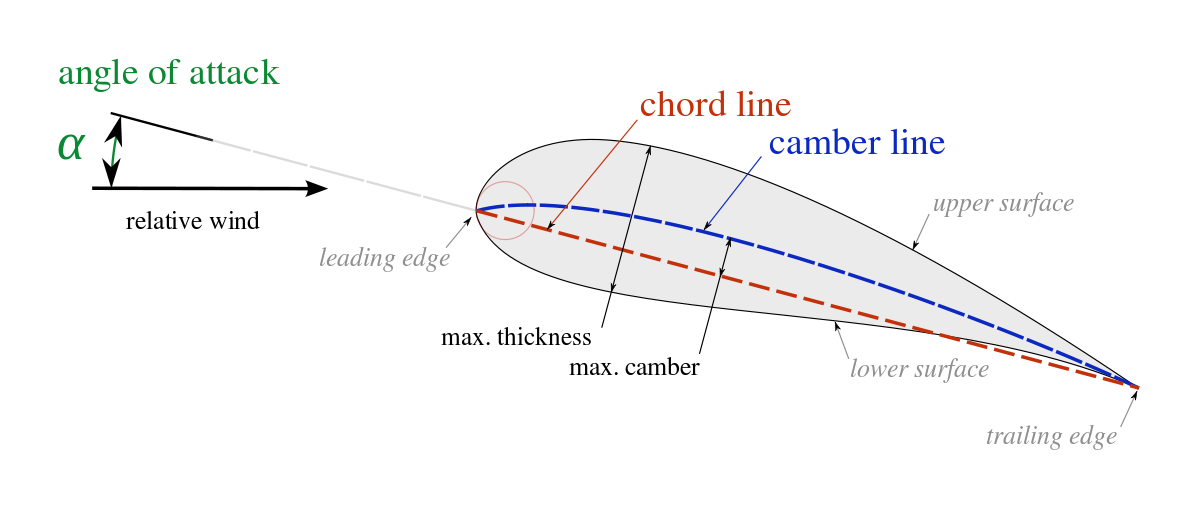
\includegraphics[scale=0.3]{diagrama-asa.png}
		\caption{Diagrama da vista lateral de uma asa}
		\label{fig:diagrama-asa}
	\end{figure}

	Além da dimensão da \emph{linha de corda}, dois parâmetros importantes de um aerofólio são o \emph{coeficiente de sustentação} $C_l$ e o \emph{coeficiente de arrasto} $C_d$, definidos por \cite{nasa:liftcoeff,nasa:dragcoeff}
	\begin{align}
		C_l = \frac{2\,L}{\rho\,w_\infty^2\,A}\label{eqn:coef-lift}\\
		C_d = \frac{2\,D}{\rho\,w_\infty^2\,A}\label{eqn:coef-drag}
	\end{align}

	Nestas equações, $\rho$ representa a massa específica do ar, $w_\infty$ é a velocidade relativa de escoamento do ar em relação ao aerofólio, $A$ é a área de superfície, e $L$ e $D$ são as forças de sustentação e arrasto, respectivamente.
	Estes valores compreendem todas as dependências complexas do comportamento do aerofólio e geralmente são determinados de maneira experimental \cite{nasa:liftcoeff}.

	\subsection{Velocidade relativa de escoamento}
	A velocidade relativa de escoamento, que já é identificada na \figurename\ \ref{fig:diagrama-asa}, é importante no estudo da pá de um aerogerador,
	já que a pá está girando, enquanto o vento incide paralelo ao seu eixo de rotação.
	Isso pode ser identificado de maneira mais fácil na \figurename\ \ref{fig:velocidades-asa}.
	No exemplo, a pá se movimenta na direção horizontal da imagem, enquanto o vento incide perpendicularmente, identificado ali pelo vetor $U_0$.
	O movimento da pá, por sua vez, provoca o aparecimento de um outro vetor de velocidade do vento, na direção perpendicular a $U_0$,
	que é identificado na imagem por $\omega r(1+a')$.
	A soma destes dois vetores resulta no vetor de velocidade relativa do vento, ilustrado como $W$.
	Nos cálculos deste documento, este vetor será representado por $w_\infty$, 
	como já pode ser visto nas Equações \ref{eqn:coef-lift} e \ref{eqn:coef-drag}.

	\begin{figure}[ht]
		\centering
		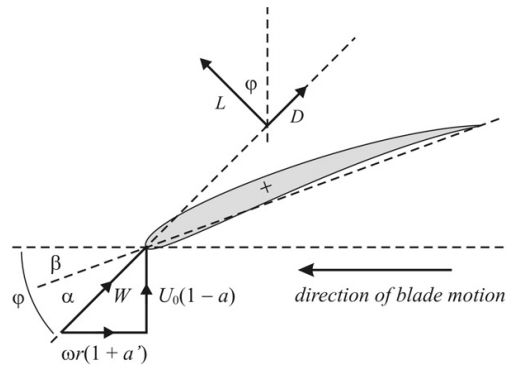
\includegraphics[scale=0.5]{diagrama-velocidades-asa.png}
		\caption{Diagrama de velocidades na pá do aerogerador}
		\label{fig:velocidades-asa}
	\end{figure}

	Outras informações importantes que podem ser extraídas da imagem são o ângulo de passo, ou \foreignlanguage{english}{pitch},
	representado por $\beta$, e o \emph{ângulo de ataque} $\alpha$.
	O primeiro compreende o ângulo entre a linha de corda da pá e a direção do deslocamento da pá, 
	enquanto $\alpha$ é o ângulo formado o vetor de velocidade relativa $w_\infty$ e a linha de corda.
	
	É importante notar que ao longo do comprimento da pá, a velocidade tangencial, calculada por $\omega\,r$, é mais alta.
	No triângulo de velocidades, é possível notar que isso provoca uma redução no ângulo de ataque $\alpha$.
	É por esse motivo que as pás de aerogeradores são \emph{torcidas}, isto é, alteram o ângulo da linha de corda ao longo do seu comprimento.

	\subsection{Forças de sustentação e arrasto}
	Embora as forças de sustentação e arrasto possam ser obtidas rearranjando as Equações \ref{eqn:coef-lift} e \ref{eqn:coef-drag}, elas podem ser representadas de forma seccional, em unidades de força por unidades de comprimento.
	Nesta forma, as equações utilizam o comprimento da linha de corda, representado por $\mathcal{C}$:
	\begin{align}
		L' = \frac{1}{2}\,\rho\,w_\infty^2\,C_l\,\mathcal{C} \\
		D' = \frac{1}{2}\,\rho\,w_\infty^2\,C_d\,\mathcal{C}
	\end{align}

	Como é possível ver na \figurename\ \ref{fig:velocidades-asa}, a força de arrasto é sempre paralela à direção relativa do vento,
	enquanto a força de sustentação atua perpendicularmente a ela.
	As componentes destas forças que atuam na direção tangencial à rotação da pá são o que colabora ao movimento do aerogerador,
	enquanto as componentes paralelas ao eixo de rotação, representam uma carga que deve ser suportada pela estrutura da pá e da torre.

	Pela sua orientação, as duas forças colaboram para ambos os efeitos, de modo que a sua decomposição pode ser feita através do
	\emph{ângulo de incidência} $\varphi$ representado na \figurename\ \ref{fig:velocidades-asa}:
	\begin{align}
		F_t' = L'\sin\varphi - D'\cos\varphi \label{eqn:forca-tangencial}\\
		F_a' = - L'\cos\varphi - D'\sin\varphi \label{eqn:forca-axial}
	\end{align}

	Aqui, estas forças também estão representadas por unidade de comprimento.
	O torque provocado pela força tangencial, que é o objeto de interesse, é obtido multiplicando a Equação \ref{eqn:forca-tangencial} 
	pelo raio local na pá e integrando sobre o comprimento da pá
	\begin{equation}
		\tau = \int_0^R F_t' \cdot r\,\mathrm{d}r
	\end{equation}
	o que resulta no torque produzido por uma pá.
	O torque total gerado é o produto desta equação pelo número de pás na turbina.

	\subsection{Controle do ângulo de passo}
	Como pôde ser visto nas equações anteriores, não há nenhuma dependência entre o ângulo de passo $\beta$
	e o torque resultante no rotor.
	É importante frisar que o ângulo de incidência $\varphi$ utilizado nas Equações \ref{eqn:forca-tangencial} e \ref{eqn:forca-axial}
	\emph{não depende} do ângulo da pá.

	A variação no ângulo passo, no entanto, tem um efeito direto no \emph{ângulo de ataque} $\alpha$ da pá.
	Esse, por sua vez, é responsável por ditar valores para os coeficientes de sustentação e arrasto,
	$C_l$ e $C_d$ \cite{spera:2008,petrilli:2009,hoffmann:1996}.

	Para cada perfil aerodinâmico, há um conjunto de curvas que definem estes coeficientes em função do ângulo de ataque.
	Normalmente, estes valores são determinados em faixas de ângulo entre $-20\degree$ e $20\degree$.
	Não é comum obter estas informações para a grande variedade de ângulos de um aerogerador, que vai até os $90\degree$.

	Em vista disso e da similaridade com os exemplos mostrados, o perfil aerodinâmico escolhido para o modelo é o \emph{NACA 4415},
	que é um aerofólio com câmber (não-simétrico), para o quais os valores dos coeficientes foram encontrados.

	\subsubsection{Curvas do coeficiente de sustentação}
	As curvas representadas nas \figurename s \ref{fig:coef-lift-angulos-altos} e \ref{fig:coef-lift-angulos-baixos},
	obtidas nas referências \cite{airfoiltools:naca4415,petrilli:2009}, mostram valores
	para o coeficiente $C_l$ em relação a valores de ângulo de ataque $\alpha$ enre $-15\degree$ e $90\degree$.

	\begin{figure}[ht]
		\centering
		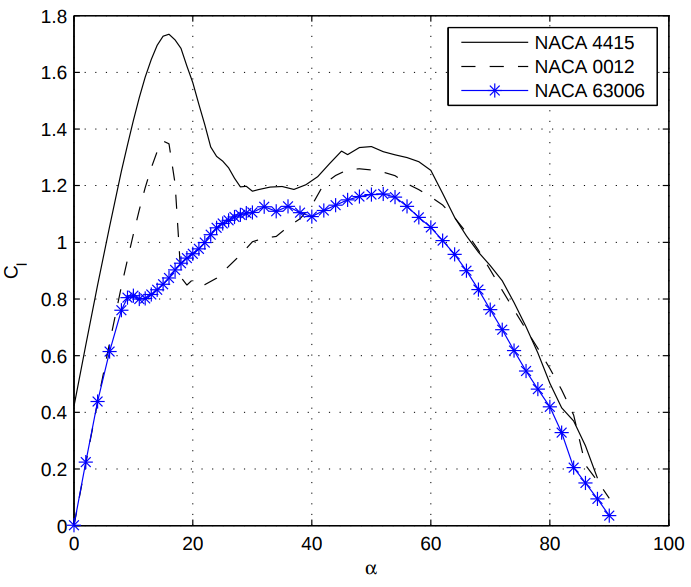
\includegraphics[scale=0.3]{coef-lift-angulos-altos.png}
		\caption{Coeficiente de sustentação para o perfil NACA 4415 (entre outros), para ângulos de 0 a 90 graus}
		\label{fig:coef-lift-angulos-altos}
	\end{figure}

	\begin{figure}[ht]
		\centering
		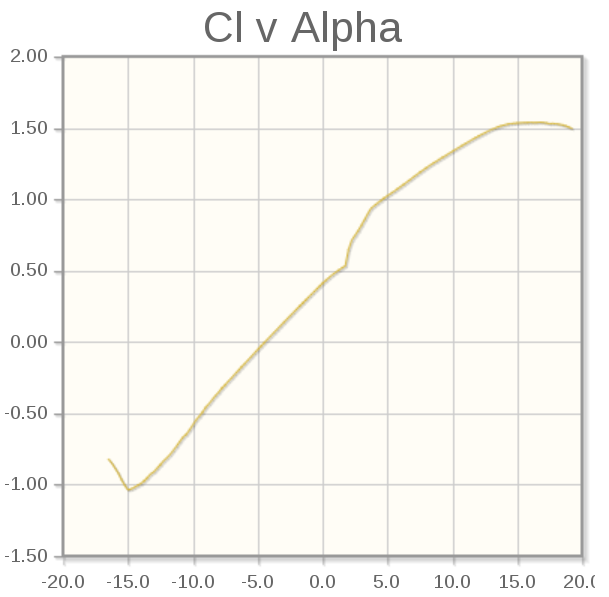
\includegraphics[scale=0.3]{coef-lift-angulos-baixos.png}
		\caption{Coeficiente de sustentação para o perfil NACA 4415, para ângulos de $-15\degree$ a $20\degree$.}
		\label{fig:coef-lift-angulos-baixos}
	\end{figure}

	Embora sejam duas curvas distintas, é visível que elas podem ser conectadas no ponto $\alpha = 0$.
	Adicionalmente, o gráfico mostrado na \figurename\ \ref{fig:coef-lift-angulos-altos} considera um número de Reynolds no escoamento
	igual a $3.000.000$.
	Na \figurename\ \ref{fig:coef-lift-angulos-baixos}, por outro lado, o valor de Reynolds considerado é $1.000.000$.
	Para valores nominais de trabalho do aerogerador, este valor seria de $1.500.000$, aproximadamente.

	\subsubsection{Curvas do coeficiente de arrasto}
	As curvas representadas nas \figurename s \ref{fig:coef-drag-angulos-altos} e \ref{fig:coef-drag-angulos-baixos},
	obtidas nas referências \cite{airfoiltools:naca4415,spera:2008}, mostram valores para o coeficiente
	$C_d$ em relação a valores de ângulo de ataque $\alpha$ entre $-15\degree$ e $110\degree$.

	\begin{figure}[ht]
		\centering
		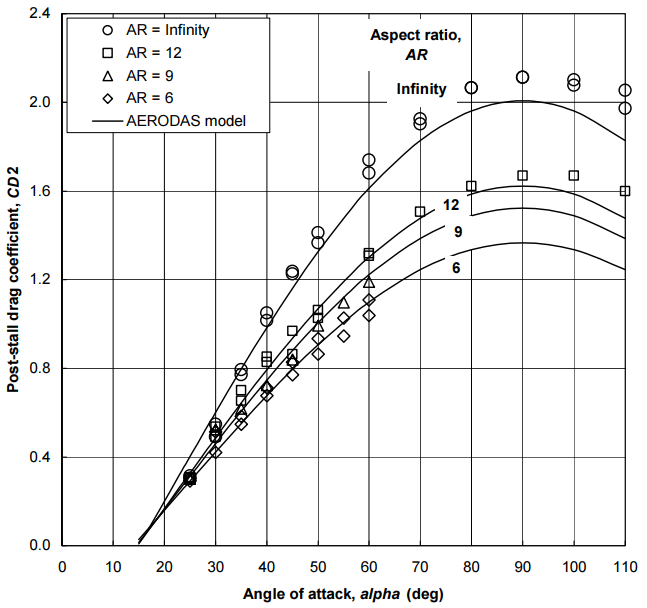
\includegraphics[scale=0.3]{coef-drag-angulos-altos.png}
		\caption{Coeficiente de arrasto para o perfil NACA 4415, para ângulos de $15\degree$ a $110\degree$.}
		\label{fig:coef-drag-angulos-altos}
	\end{figure}

	\begin{figure}[ht]
		\centering
		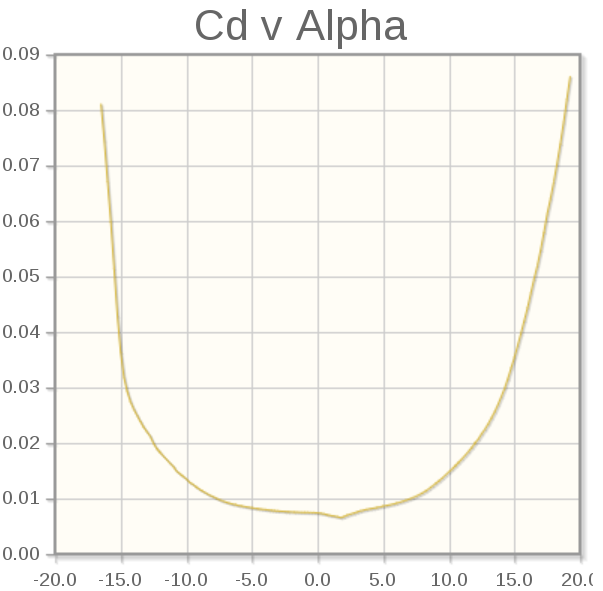
\includegraphics[scale=0.3]{coef-drag-angulos-baixos.png}
		\caption{Coeficiente de arrasto para o perfil NACA 4415, para ângulos de $-15\degree$ a $20\degree$.}
		\label{fig:coef-drag-angulos-baixos}
	\end{figure}

	A \figurename\ \ref{fig:coef-drag-angulos-altos} mostra diferentes curvas, que representam os coeficientes de arrasto para o perfil NACA 4415
	sob as mesmas condições de escoamento, mas com diferentes \emph{alongamentos} (ou \foreignlanguage{english}{aspect ratio}) no aerofólio.
	Esta medida representa a razão entre a envergadura e o comprimento de corda.

	\section{Aerogerador utilizado}
	Todo o \emph{software} desenvolvido e os modelos criados utilizam como base um gerador Enercon E-82 E2 de 2 MW de potência.
	Os dados técnicos da turbina eólica são exibidos na Tabela \ref{tab:dados-tecnicos} \cite{enercon:e82}.
	\begin{table}[ht]
		\centering
		\begin{tabular}{l|r|l}
			\textbf{Característica} & \textbf{Valor} & \textbf{Unidade}\\ \hline
			Potência nominal & $2000$ & kW\\ \hline
			Velocidade nominal do vento & $14$ & m/s \\ \hline
			Velocidade de vento de início de operação & $2,5$ & m/s \\ \hline
			Velocidade de parada (controle de tempestade não ativado) & $25$ & m/s \\ \hline
			Velocidade de rotação do rotor com geração de energia & $6 \text{~a~} 18$ & rpm \\ \hline
			Diâmetro & $82$ & m \\ \hline
			Área varrida pelas pás & $5281$ & m\textsuperscript{2} \\ \hline
		\end{tabular}
		\caption{Dados técnicos do aerogerador Enercon E-82 E2}
		\label{tab:dados-tecnicos}
	\end{table}
	\clearpage
	
	\bibliography{Bibliografia}
	
\end{document}
